\documentclass[graphics]{beamer}

\usepackage{graphicx}
\usepackage{verbatim}
\usepackage{wrapfig}
\useoutertheme{shadow}
%\usecolortheme{orchid}
\usecolortheme{seahorse}


% math commands
\newcommand{\be}{\begin{eqnarray}}
\newcommand{\ee}{\end{eqnarray}}
\newcommand{\beq}{\begin{equation}}
\newcommand{\eeq}{\end{equation}}
\def\simless{\mathbin{\lower 3pt\hbox
      {$\rlap{\raise 5pt\hbox{$\char'074$}}\mathchar"7218$}}}
\def\simgreat{\mathbin{\lower 3pt\hbox
      {$\rlap{\raise 5pt\hbox{$\char'076$}}\mathchar"7218$}}} %> or of order

% variables

\def\toonscale{0.45}
\def\mboxy#1{\mbox{\small #1}}


\begin{comment}
\AtBeginSection[]{
  \frame{
    \frametitle{Outline}
    \tableofcontents[currentsection]
  }
}
\end{comment}

\title{Wave Optice lensing
}
%\subtitle{interim update}
\author[U. Pen]{Ue-Li Pen
\\ Dylan Jow, Job Feldbrugge, Neil Turok 
}
\date{May 18, 2021}


\begin{document}

%\section*{Introduction}
\section{Lenses}

\begin{comment}
  \subsection{Outline}

  \frame{
    \frametitle{Outline}
    \tableofcontents
  }
\end{comment}

\frame{\maketitle}



  \frame{
    \frametitle{Lenses}
    \begin{itemize}
        \item Gravitational Lensing: micro, macro
        \item Plasma lensing
        \item Coherent sources: forms interference pattern
        \item expected (observed) for FRBs
        \item 
        \item 
        \item 
    \end{itemize}
  }


  \frame{
\vspace{-0.5in}
    \frametitle{History}
    \begin{itemize}
    \item Huygens, Fermat, 
    \item Picard-Lefschitz (19th century), Witten (2010)          
        \item concept: Oscillatory path integral
        \item 
        \item imaginary images
        \item 
            
    \end{itemize}
  }


  \frame{
\vspace{-0.5in}
    \frametitle{Optics: Geometric, Eikonal, Wave, P-L}
    \begin{itemize}
        \item Consider 1-D lens
        \item potential lensing function $\Psi(\theta)$
        \item deflection $\Psi'$
    \end{itemize}
\vspace{-1in}\hspace{2.5in}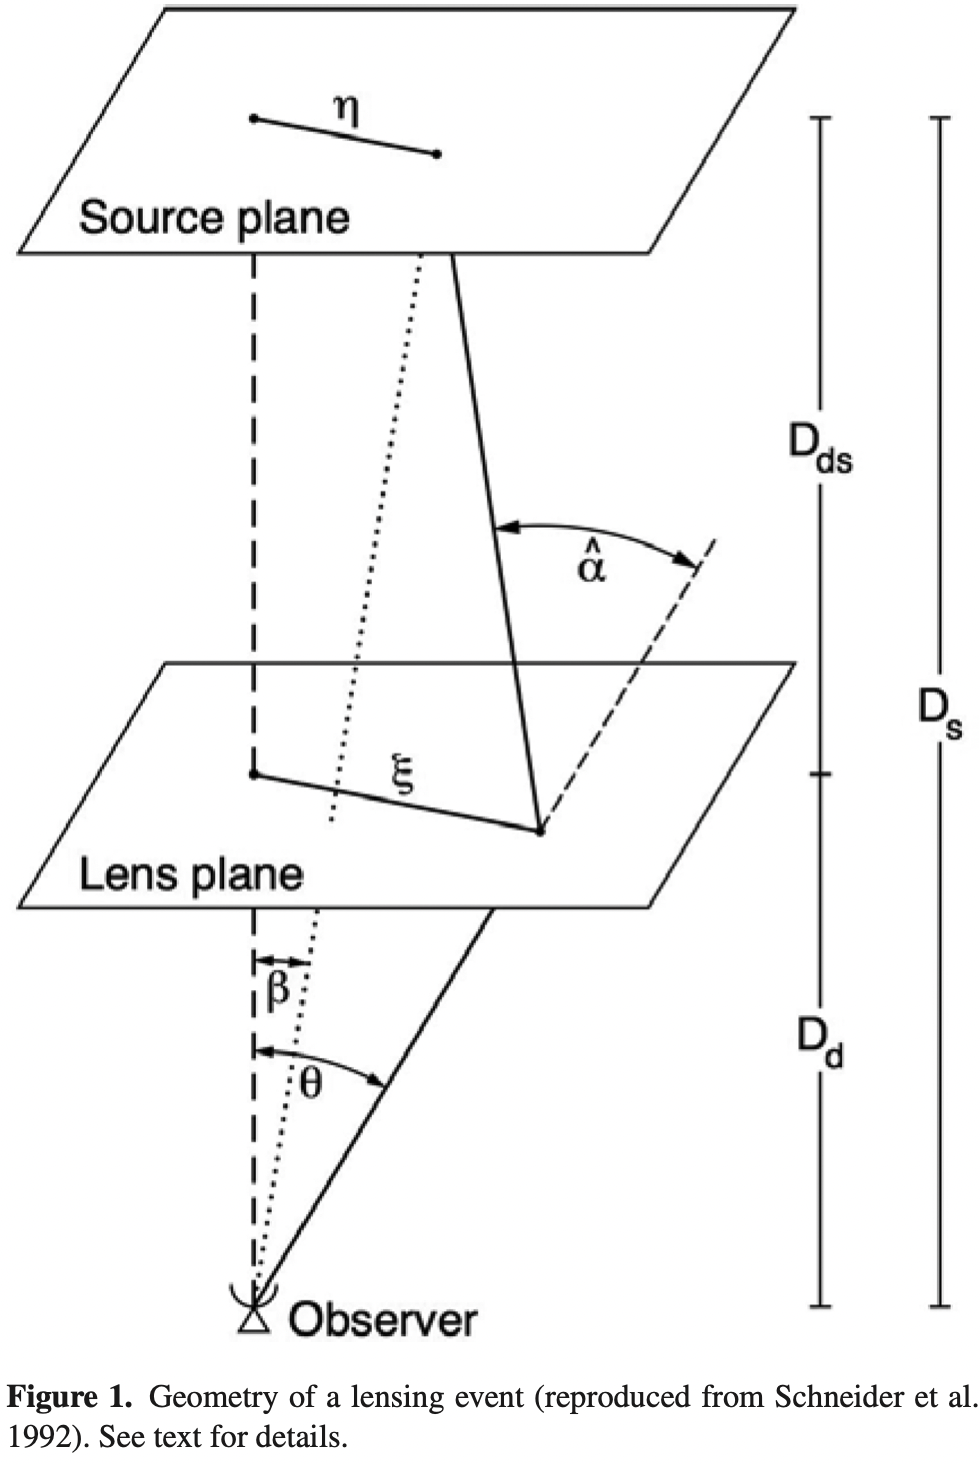
\includegraphics[width=1.5in]{Figures/lens.png}

  }


  \frame{
\vspace{-0.5in}
    \frametitle{Huygen's Principle: Path Integral}
    \begin{itemize}
        \item $A=\int e^{i S(\theta,\mu)} d\theta$ 
        \item $S=\nu (\theta^2+\Psi)$
        \item Highly oscillatory integral, even for $\Psi=0$
        \item Stationary phase points: $\partial_\theta S=0$ leads to
          Eikonal images $\theta_i$.
        \item Geometric limit considers only {\it Real} $\theta_i$ and
          absolute value of the action $S$, giving up phase
          information
        \item Geometric optics applicable at short wavelengths
          (e.g. optical gravitational lensing of finite size sources,
          e.g. stars)          
    \end{itemize}
  }

  \frame{
\vspace{-0.5in}
    \frametitle{Imaginary Images}
    \begin{itemize}
    \item consider ``rational lens'' potential $\psi(\theta)=\alpha/(1+x^2)$
    \item Geometric/eikonal images at $\psi'=x$
    \item 5 roots.  1 or 3 real roots, rest imaginary
    \item P-L: at most one imaginary image contributes!
    \item imaginary image can be brighter than unlensed real image
    \end{itemize}
  }


  \frame{
%\vspace{-0.5in}
    \frametitle{Rational 1-D lens}
\begin{center}
\includegraphics[width=3.1in]{Figures/theta-beta.eps}
\end{center}
  }

  \frame{
\vspace{-0.5in}
    \frametitle{Picard-Lefschetz Theory}
    \begin{itemize}
    \item descend integral along real line along morse function Im(S)
    \item contour deforms into finite number of Thimbles of constant
      phase with maximum at saddle point (extrema $dS=0$)
    \item correctly identifies relevant saddle points
    \item resolves numerical challenges of oscillatory integral
    \item complex analysis works in multiple variables
    \item elevates concept of ``image'' deep into wave optics
    \item multiple public implementations (Feldbrugge+, Jow+)
    \end{itemize}
  }



  \frame{
\vspace{-0.5in}
    \frametitle{Picard-Lefschetz Theory}

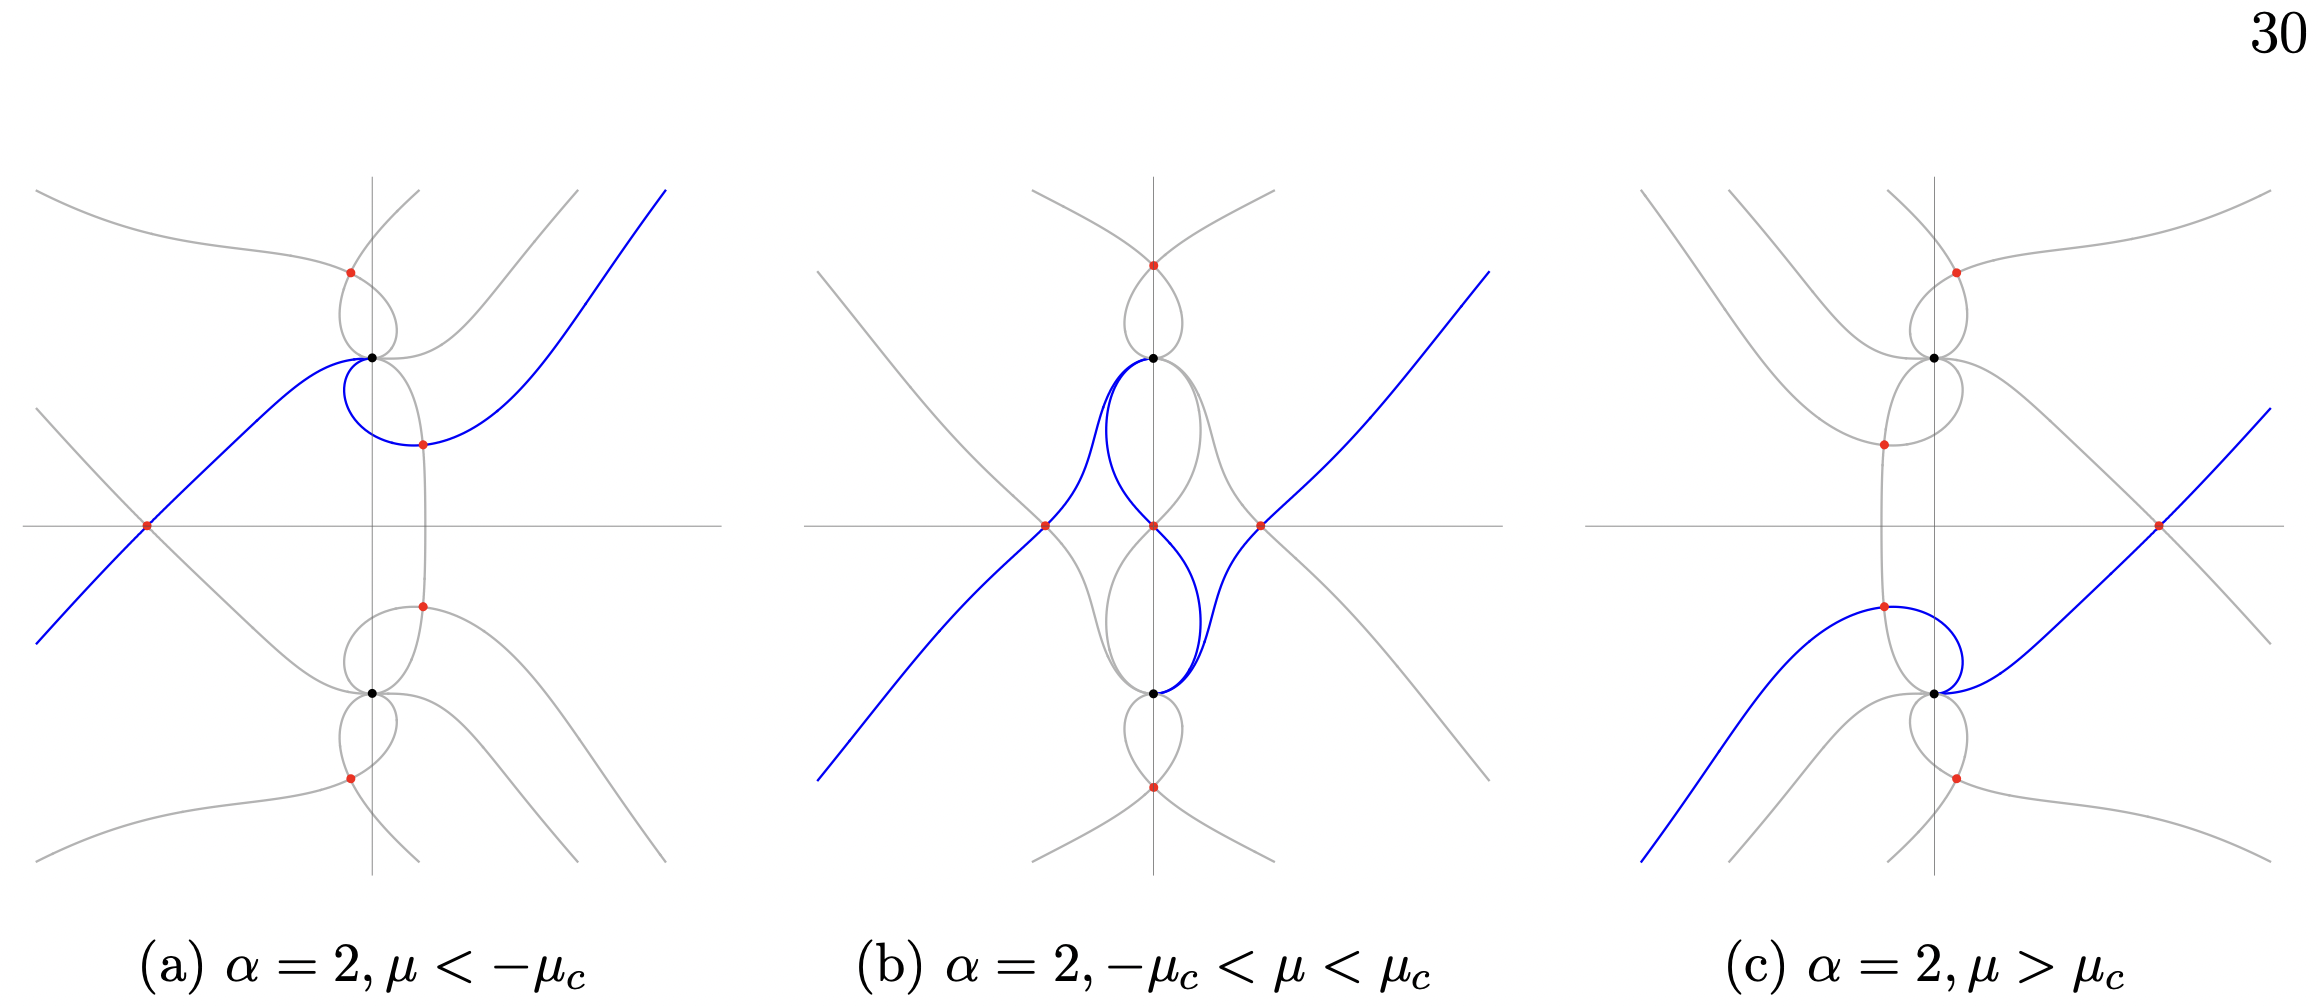
\includegraphics[width=4.5in]{Figures/thimbles.png}

Feldbrugge+2019
  }


  \frame{
\vspace{-0.5in}
    \frametitle{New Observables}
    \begin{itemize}
    \item weak lensing: imaginary image allows time delay measurement
    \item strong lensing: delay measurements enable measurement of co-linearity
    \item microlensing: instant time delay, planets
    \item macrolensing: potentially nano-second delay -- universe expands!
    \item dimensionless strain picoseconds/years $h\sim \Delta t/t \sim 10^{-20}$:
      competitive with LIGO, etc
    \item          
    \end{itemize}
  }



  \frame{
\vspace{-0.5in}
    \frametitle{Stokes Phenomenon}
    \begin{itemize}
    \item Imaginary images (dis-)appear at caustics and Stokes lines
    \item Caustic: 
    \item 
    \item 
    \item 
    \item 
    \end{itemize}
  }

  \frame{
\vspace{-0.5in}
    \frametitle{Macrolensing}
    \begin{itemize}
    \item Wucknitz+ 2021
    \item alternate approach to cosmography
    \item triangulation: lens model+time delay measurement = $H_0$
    \item weak link has been lens model
    \item Wave optics: time delay observable to nanoseconds
    \item 
    \end{itemize}
  }



  \frame{
\vspace{-0.5in}
    \frametitle{Discussion}
    \begin{itemize}
    \item Eikonal effects applicable to compact radio sources,
      e.g. FRBs, pulsars
    \item full wave
effect dominates for long wavelengths as Fresnel scale is bigger then Einstein radius
    \item radio waves: planets
    \item gravitational waves: stars (LIGO) galaxies (PTA)
    \item 
    \item 
    \item 
    \end{itemize}
  }



  \frame{
\vspace{-0.5in}
    \frametitle{Current status}
    \begin{itemize}
    \item Eikonal: pulsar scintillation, wind magnification (Main+ 2018)
    \item full wave optics: pulsar wind lensing, solar wind (IPS)
    \item 
    \item 
    \item 
    \item 
    \item 
    \end{itemize}
  }



  \frame{
\vspace{-0.5in}
    \frametitle{Conclusions}
    \begin{itemize}
    \item wave optics changes nature of observables: potentially most
      precise measurements in physics
    \item coherent radio waves (FRBs, pulsars): described by Eikonal
      away from caustics/catastrophies
    \item long wavelength GW (LIGO, LISA, PTA): full wave effects, P-L theory
    \item importance of imaginary images
    \item 
    \item 
    \item 
    \end{itemize}
  }

\end{document}
